% Name: Graph and its adjacency matrix
% Description: A small undirected graph beside its adjacency matrix, with a 1 wherever two vertices share an edge.
% Tags: adjacency matrix, graph, representation, linear algebra

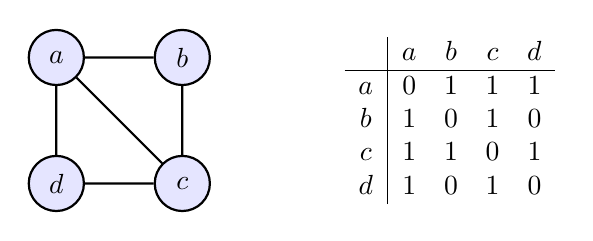
\begin{tikzpicture}[v/.style={circle, draw, thick, fill=blue!10, minimum size=7mm, inner sep=0pt}]
  \node[v] (a) at (0,1.6) {$a$};
  \node[v] (b) at (1.6,1.6) {$b$};
  \node[v] (c) at (1.6,0) {$c$};
  \node[v] (d) at (0,0) {$d$};
  \draw[thick] (a) -- (b) (b) -- (c) (c) -- (d) (d) -- (a) (a) -- (c);
  \node at (5,0.8) {$
    \begin{array}{c|cccc}
        & a & b & c & d \\ \hline
      a & 0 & 1 & 1 & 1 \\
      b & 1 & 0 & 1 & 0 \\
      c & 1 & 1 & 0 & 1 \\
      d & 1 & 0 & 1 & 0
    \end{array}
  $};
\end{tikzpicture}
